\chapter{Stand des Wissens und der Technik}
Für den Grundaufbau der Messmethodik ist das Grundwissen über einzelne Elemente unverzichtbar. In diesem Kapitel wird auf spezifisch ausgewählte Punkte eingegangen, um das Verständnis weiterer Zusammenhänge für den Leser zu vereinfachen.


\section{Funktionsweise eines Prozessors}

Ein Prozessor ist eine universelle Rechenmaschine, die sich durch eine definierte Reihe von Anweisungen programmieren lässt. Zu den arithmetischen Anweisungen gehören der Zugriff auf Speicheradressen und Sprünge innerhalb der Abfolge der Anweisungen.
Bereits der britische Mathematiker Alan Turing konnte aufzeigen, dass ein universelles Berechnungsmodell umsetzbar ist, wenn ein Rechner neben dem Speicherzugriff auch Sprunganweisungen innerhalb des Programmcode durchführen und an einer definierte Stelle die Ausführung fortsetzt kann\cite{Hoffmann2014l}. Auf diesen besonderen Eigenschaften bauen die heutigen Prozessoren auf. Ein Programm, das den Prozessor ansteuert, besteht aus einer endlichen Anzahl von geordneten Anweisungen. Der Prozessor befolgt, streng nach dem Ablauf, Anweisung für Anweisung. Diese ablaufenden Anweisungen können dabei auch Sprünge zu anderen Stellen innerhalb des Programms definieren.
\par
Die Prozessoren, auch Zentraleinheiten oder CPUs genannt, besitzen im Inneren drei Einheiten, die über einen Datenbus verbunden sind. Dies ist in der \autoref{fig:CPU} ersichtlich. Dabei kann der Datenbus je nach Grösse oder Leistung der CPU variieren. Die zurzeit meist verbreiteten CPUs, die in PCs verbaut sind, verwenden einen 64bit-Datenbus. In dieser Arbeit wird aber mit kleineren CPUs, die lediglich einen 32bit-Datenbus besitzen, gearbeitet. Die Control Unit\cite{patterson2013computer} ist dafür verantwortlich, dass das Programm immer an der richtigen Stelle ausgeführt wird. Sie nimmt Anweisungen entgegen, dekodiert diese und übergibt sie der Arithmetic Logic Unit (ALU). Die Übergabe der Daten an die ALU und die Register erfolgt durch die Weichenstellung des Datenbusses. Die ALU ermöglicht es, Rechen- sowie logische Operationen an den Daten auszuführen. Die Register haben die Grösse des Datenbusses und dienen dazu, die Daten von und zur ALU zu bewegen. Eine CPU besitzt mehrere Register, die je nach CPU-Architektur variieren. Die Register lassen sich in zwei Kategorien, Universal- und Hilfsregister, unterteilen. In den Universalregistern lassen sich die zu bearbeitenden Daten speichern. Die Hilfsregister haben je nach ihrer Funktion eine besondere Rolle zugeordnet erhalten. Beispielsweise zählt das Statusregister zu den Hilfsregistern. Dieses spezielle Hilfsregister gibt Aufschluss über das Resultat der vorherigen Operation. So lässt sich über dieses Hilfsregisters herauslesen, ob eine Operation von zwei Zahlen den möglichen Speicherplatz des Registers übersteigt und es zu einem sogenannten "overflow" kommt.
Da die Anzahl Universalregister meist sehr klein ist, müssen die Daten immer wieder von den Universalregistern in den RAM und zurückgeladen werden.



\begin{comment}
Useful example for Pipelining

It may take X hours to build a single car, but if you start building a car then 30 seconds later start building another and every 30 seconds start another then after X hours you will have a new car every 30 seconds. Does that mean it takes 30 seconds to make a car? Of course not. But it does mean that once up and running you can average a new car every 30 seconds on that production line.

More info:
https://books.google.ch/books?id=PSonZP4Nj5sC&pg=PA11&lpg=PA11&dq=raspberry+half+cpu+cycle&source=bl&ots=m_3q-usqla&sig=Ub9KeDbuSkCLgFGSRyFc_KZs7Ow&hl=en&sa=X&ved=0ahUKEwj89Pa6iZnNAhXEiRoKHRtUALcQ6AEIMTAC#v=onepage&q=raspberry%20half%20cpu%20cycle&f=false
\end{comment}



\begin{figure}[t]
\centering
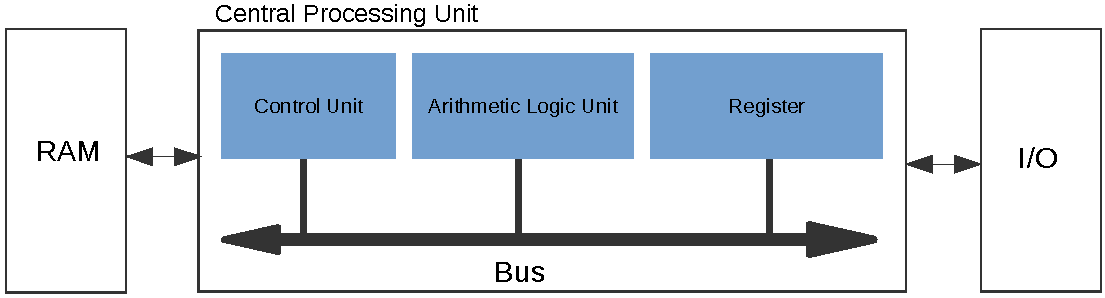
\includegraphics[width=1.0\textwidth]{images/cpu.pdf}
\caption{Central Processing Unit}
\label{fig:CPU}
\end{figure}

\section{Aufbau des Linux Betriebssystems}
% Monolithische Systeme 
% TRAP-Instruktion

Inspiriert durch das Betriebssystem Minix, das von Andrew S. Tanenbaum für Ausbildungszwecke erstellt wurde, machte es sich Linus Torvalds zum Ziel, dieses vollwertige System neu zu schreiben. Im Jahr 1991 erschien die erste Linux Version 0.01\cite{ehses2011systemprogrammierung_chap2}. Heute ist es ein weit verbreitetes Betriebssystem, das für unterschiedlichen Anwendungszwecke wie für Desktops, Server, Smartphones und Embedded Systems eingesetzt wird.
\par
Die Aufgabe des Betriebssystemkerns, der meistens einfach nur Kernel genannt wird, ist es, eine Softwareschicht zwischen Hardware und Programm zu erstellen. Die Programme haben somit keinen direkten Zugriff auf die Hardware. Jedes Programm, das Informationen der Hardware benötigt, muss durch die Schicht des Kernels gehen. Die Kommunikationen zwischen Programm und Kernel werden Systemaufrufe (engl. Systemcalls) genannt. Die unterschiedlichen Systemaufrufe sind im POSIX standardisiert\cite{ehses2011systemprogrammierung_chap2}. Zusätzlich erstellt der Kernel eine Art Abkapselung eines Programms. Dadurch können mehrere Programme gleichzeitig laufen, ohne dass das eine Programm Zugriff auf das andere hat. Der Kernel verteilt die freien Ressourcen der CPU abwechslungsweise an die Programme. Dieses Verfahren heisst Multitasking und wurde seit den Anfängen unterstützt.
\par
Durch die zusätzliche Softwareschicht, die der Kernel bietet, müssen Programmierer ein Programm nicht für eine bestimmte Hardware schreiben, sondern für ein bestimmtes Betriebssystem. Dies ermöglicht eine höhere Portabilität eines Programms. Hardware wie Festplatten oder Netzwerkcontroller werden vom Kernel vereinheitlicht und dem Programm durch Systemaufrufe zur Verfügung gestellt.
\par

\begin{wrapfigure}{L}{0.49\textwidth}
\centering
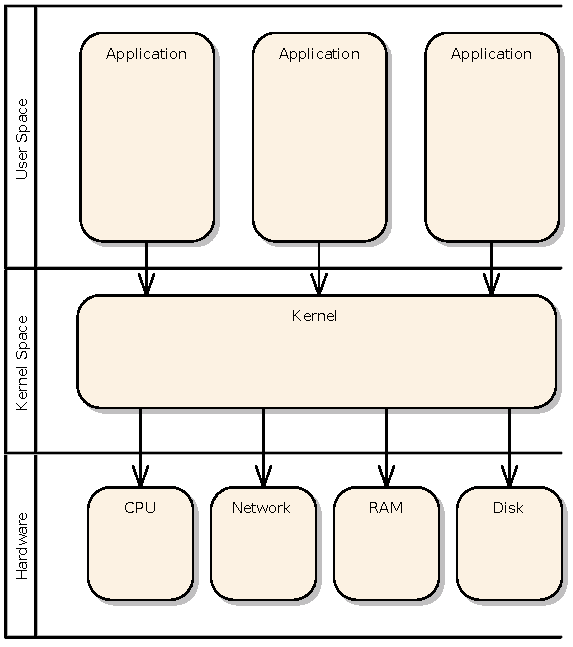
\includegraphics[scale=0.8]{images/kernel.pdf}
\caption{Linux Kernel}
\label{fig:kernel}
\end{wrapfigure}

Die \autoref{fig:kernel} zeigt, wie die unterschiedlichen Schichten miteinander kommunizieren. Eine Anwendung wird ausschliesslich im Benutzermodus (engl. User Space) ausgeführt. Durch Systemaufrufe werden Anfragen an den Kernel übermittelt. Dabei findet ein Kontextwechsel vom unprivilegierten in den privilegierten Modus statt. Der unprivilegierte Modus bezeichnet den Benutzermodus, in dem eine Applikation nur beschränkt über den Arbeitsspeicher verfügen kann und nur gewisse CPU-Befehlssätze ausgeführt werden können. Dies stellt sicher, dass eine Applikation gegenüber dem Rest des Systems abgekapselt betrieben wird und nicht darauf zugreifen kann. Nach dem Systemaufruf geht der Prozessor in den privilegierten Modus über und der Kernel trägt die Verantwortung, die Anfrage im Kernelmodus (engl. Kernel Space) zu verarbeiten. Der Kernelmodus weist im Gegensatz zum Benutzermodus keine Einschränkungen auf und hat deswegen auch Zugang zur Hardware und zum gesamten Arbeitsspeicher. Demzufolge dient der Kontextwechsel dazu, dass derjenige Programmcode, der nicht zum Kernel gehört, nur in einem unprivilegierten Modus ausgeführt werden kann.


\section{Unterschiede zwischen CISC- und RISC-CPUs\cite{Hoffmann2014_risc_cisc}}

Die CPUs können, je nach dem wie ihre Befehlssatzarchitektur aufgebaut ist, in unterschiedliche Gruppen aufgeteilt werden. CISC-Prozessoren (Custom Instruction Set Computer) weisen im Vergleich zu RISC-Prozessoren (Reduced Instruction Set Computer) sehr komplexe und umfangreiche Befehlssätze auf.
\par
Im Jahr 1978 führte Intel mit dem 8086 Prozessor den x86-Befehlssatz ein. Dieser wurde zum Urvater moderner CISC-Prozessoren. Schon damals besass dieser Prozessor zirka 120 Befehlssätze. Im Verlauf der Jahre zeichneten sich die CISC-Prozessoren durch immer mehr und komplexere Befehlssätze aus. Dabei wurde stets darauf geachtet, dass die Architektur der neueren Modelle rückwärtskompatibel ausgestaltet ist, damit ältere Software auch ohne Anpassung auf neueren Prozessoren laufen kann. Die CISC-Architektur erlaubt es, komplexe Instruktionen in einem Befehlssatz zu schreiben. Dabei wird der Befehlssatz von der CPU dekodiert und in einem oder mehreren Taktzyklen ausgeführt. Die Komplexität der Befehlssätze geht so weit, dass sogar Hardwareschleifen möglich werden. Weiter kann ein Befehlssatz die Anweisung erhalten, Daten von einer Speicherzelle im RAM direkt zu einer anderen zu transferieren, ohne dabei auf ein Register angewiesen zu sein. Daher verfügen die meisten CISC-Prozessoren in der Regel über eine geringere Anzahl von Register als RISC-Prozessoren. Zusätzlich besitzen die gegenwärtigen CISC-Prozessoren sehr umfassende Steuerwerke, damit sie die immer komplexeren Befehlssätze dekodieren und in Instruktionen aufteilen können. Die Steuerwerke dieser Prozessoren bestehen normalerweise aus Hardware-Implementationen. Jedoch können sie innerhalb des Steuerwerks ebenso Microcode, also eine Software-Implementation, aufweisen.
\par
Bis Mitte der Achtziger war man der Meinung, dass durch komplexere Hardware und die damit verbundene höhere Anzahl an verfügbaren Befehlssätzen eine grössere Leistung erzielt werden kann. Der Trend zu immer mehr und vielfältigeren Befehlssätzen nahm aber ab. Dies hat zur Folge, dass heute einerseits kaum noch Programme in Assembler geschrieben und andererseits die gängigen Compiler so gebaut werden, dass sie nur noch etwa 20 Prozent der Befehlssätze benötigen. Dazu kommt, dass die komplexen Verarbeitungsstrukturen innerhalb eines CISC-Prozessors die Elementaroperationen verlangsamen.
\par
Patterson, David A. und Sequin, Carlo H. prägten zwar Ende der achtziger Jahre den Begriff "RISC" \cite{Patterson:1981:RIR:800052.801895}, jedoch existierten diese Art der Prozessoren mit einfacher Architektur bereits seit geraumer Zeit. Die Technik war noch nicht sehr ausgereift und die Prozessoren konnten nur eine begrenzte Anzahl an Instruktionen verarbeiten. RISC-Prozessoren zeichnen sich durch eine Load-and-Store-Architektur, eine höhere Menge an Universalregistern und die Begrenzung auf Elementarinstruktionen aus. Der Begriff "Load and Store" meint, dass Daten stets über Register geladen und gespeichert werden müssen. Demnach ist es bei dieser Architektur nicht möglich, die Daten von einer Speicherzelle im RAM zu einer anderen zu transferieren, ohne sie zuerst in einem Register zwischenzuspeichern. Es benötigt bei diesem Vorgehen somit immer mindestens zwei Taktzyklen; den ersten zum Laden der Daten in ein Zwischenregister und den zweiten zum Abspeichern dieser in eine andere Speicherzelle. Aufgrund der grösseren Anzahl an Registern muss ein RISC-Prozessor bei der Ausführung von Instruktionen daher weniger auf den Speicher zurückgreifen als ein CISC-Prozessor.
\par
Die frühere klassische Trennung zwischen CISC- und RISC-Prozessoren wird immer wie kleiner. Die Entwicklung der CISC-Prozessoren hat sich stark an derjenigen von RISC-Prozessoren ausgerichtet, da sie intern praktisch mit einer RISC-Struktur und einer hochentwickelten Vorverarbeitungsstufe ausgestattet sind. Bereits der Pentium Pro war mit einem RISC-Kern ausgestattet und die von aussen ersichtliche x86-Schnittstelle war, so zu sagen, ein vorgeschalteter x86-Emulator.



%\section{Energy Storage in a Capacitor}
%Grundlage Technische Informatik Kap. Halbleitertechnik lesen!

\begin{comment}

\section{Relevanz für das Experiment}

In dieser Arbeit ist die Funktionsweise der ALU relevant. Wir wissen, dass die ALU eine Reihe von Anweisungen erhält und somit jeden erdenklichen Algorithmus ausführen kann. Die ALU sowie der gesamte Prozessor sind als elektronische Schaltkreise realisiert, die Operationen auf binäre Ebene ausführen können. Die Schaltkreise werden durch die Halbleitertechnologie hergestellt. Die Millionen von witzigen Transistoren, die ein Prozessor beinhaltet, werden zu logischen Bausteinen verdrahtet. Diese logische Bausteine bestehend aus AND-, OR- und NAND-Gattern und werden innerhalb des CPU so zusammengestellt, dass sie sehr aufwändige Operationen ausführen können. Entsprechend der Operation sind eine gewisse Anzahl Transistoren im Einsatz die den Schaltkreis bilden. Je nach Grösse und Konzeption der Schaltkreise variiert die nötige Leistung für den Betrieb. Das in dieser Arbeit erstellte Experiment soll zeigen wie gross der Energieverbrauch ist für eine Bestimmte Operation die in der ALU statt findet.

\end{comment}

\section{Eingesetzte Programmiersprachen und Kompilation\cite{Bernstein2015}}

Die Benchmarks wurden in den Programmiersprachen C und Assembler geschrieben. C und Assembler sind sehr hardwarenahe Programmiersprachen. Im Vergleich zu heutigen Hochsprachen wie Java oder Python, muss sich der Programmierer mit der Hardware und dessen Funktionsweise auskennen. Eine Programmiersprache kann als Schnittstelle zwischen Mensch und Maschine betrachtet werden. Den der CPU wird diese Sprachen nicht direkt verstehen, weshalb sie zuerst in Maschinencode übersetzt werden müssen. Für ein Mensch ist aber Maschinencode zu interpretieren oder zu schreiben praktisch eine unmögliche Angelegenheit. Deshalb wird ein Programm immer in einer Programmiersprache geschrieben, das man als Sourcecode bezeichnet. Der Compiler übernimmt die Arbeit der Übersetzung und erzeugt aus dem Sourcecode Maschinencode. Dieser Vorgang heisst kompilieren. Der Compiler muss für die Erstellung von Maschinencode die CPU-Architektur auf dem das Programm später ausgeführt wird kennen. Dabei stellt er für diese Architektur spezifischen Maschinencode. Man nennt es cross-kompilieren wenn ein Compiler Maschinencode erstellt für die spätere Ausführung auf eine andere Maschine als die der Compiler ausgeführt wurde.
\par
Assembler ist eine Programmiersprache die aus Mnemotechnik (Eselsbrücken) besteht. Jede Operation die die CPU ausgeführt werden muss, werden durch Schlüsselwörter wie MOV, ADD, SUB geschrieben. Zu jedem Schlüsselwort kommen Daten, Adressen oder Registern hinzu die innerhalb dieser Operation zum verarbeiten sind. Der Compiler übersetzt die Anweisungen in Binärencode und erstellt so den gewünschten Maschinencode zusammen. Weil sich der Sourcecode von Assembler nur aus einer Abfolge von Anweisungen besteht, sind einfache Ausdrücke wie $x = 2 + 3 * 4$ bereist mit viel Aufwand verbunden. Der Programmierer muss bei Assembler die CPU-Architektur kennen und schreibt für diese ein spezifisches Assemblerprogramm. Daher sind die Programme die in Assembler geschrieben worden sind, nicht portierbar. Heute wird durch die hohe Komplexität und schlechte Portiebarkeit kaum noch in Assembler programmiert. Assembler wird nur noch dort eingesetzt wo die Kontrolle über den Ablauf des Programm gewährleistet werden muss, weil die spezifizierten Befehlssätze die einzelnen CPU-Architekturen direkt abbilden.
\par
Die C Programmiersprache 










